\documentclass[11pt,harvard]{article}
\usepackage[letterpaper, top=1in, bottom=1in, left=1in, right=1in]{geometry}
\usepackage{graphicx}
\usepackage[sort]{natbib}
\usepackage{amssymb}
\usepackage{amsmath}
\usepackage{setspace}
\usepackage{url}
\usepackage{pdflscape}
\usepackage{longtable}
\usepackage{threeparttable, booktabs}
\usepackage[export]{adjustbox}
\usepackage{enumitem}
\usepackage{comment}
\usepackage{subcaption}
\usepackage{lmodern}
\usepackage[T1]{fontenc}
\usepackage{setspace} % Load the setspace package
\usepackage{parskip} % Load the parskip package
\usepackage{float}
\usepackage{subcaption}
\usepackage{hyperref}
\usepackage[table,xcdraw]{xcolor}


\title{Sampling for the rCARI Validation Study - Mauritania (MTN)} 
\author{- rCARI Study Team - WFP, ROME - 	\\	\\For enquiries contact:\\	\\alirah.weyori@wfp.org or lena.hohfeld@wfp.org} 
\date{\today}



\begin{document}
	\maketitle \vspace{-2cm}
	\onehalfspacing
	\pagebreak
	\setlength{\parskip}{8pt} % Set the desired space before and after paragraphs
	
	% -------	
	\section{Background}
	
	The rCARI validation study is a global research project commissioned by WFP and funded by the BHA to investigate and compare remote and face-to-face (F2F) modules of the consolidated approach for reporting food insecurity (CARI). 
	The overall goal of the study is to understand to what extent food insecurity reported by rCARI is comparable or compatible with the standard CARI. Both phone (remote) and face-to-face (F2F) data collection modules \& methodologies for collecting food insecurity will used in the study.  
	
	This document outlines the study methodology, specifically the sampling process adjusted for country specific context of Mauritania. The study has been designed and implemented as a survey experiment with stratified sample selected across 2 regions (ADMIN1) in each pilot country.  
	
	\section{Overall sampling design for the rCARI Pilot}
	
	The following considerations underpin the study areas and final sample selection.
	
	\begin{itemize}[left=2.0em]
		\item Phone ownership \& accessibility within the pilot country
		\item Distribution of food insecurity
		\item Areas of accessibility taking adjusting for difference in livelihoods
	\end{itemize} 
	
	It is important to emphasize that the purpose of data collection for this study is not to produce population-level estimates but rather to compare the two methodologies with the same comparable population. While it is desirable to collect data from a variety of livelihood zones in both urban and rural communities to assess the impact of these differences with respect to modality, national coverage and representativeness is not the primary objective of the current study. 
	
	Figure 1 below presents the generic study sampling procedure. As mention earlier, selection and inclusion of study area followed a 3-point criterium: i.e., 1) phone coverage, 2) accessibility, and 3) food security situation. Phone coverage is an important consideration allowing for equal probability of reaching an equal number of households for both remote and F2F interviews, while field accessibility ensures that enumerators can successfully access and interview households in face-to-face. The food security consideration would ensure that areas that have different AFI (acute food insecurity) situations are adequately represented in the study sample. 
	
	\begin{figure}[H]
		\begin{center}
			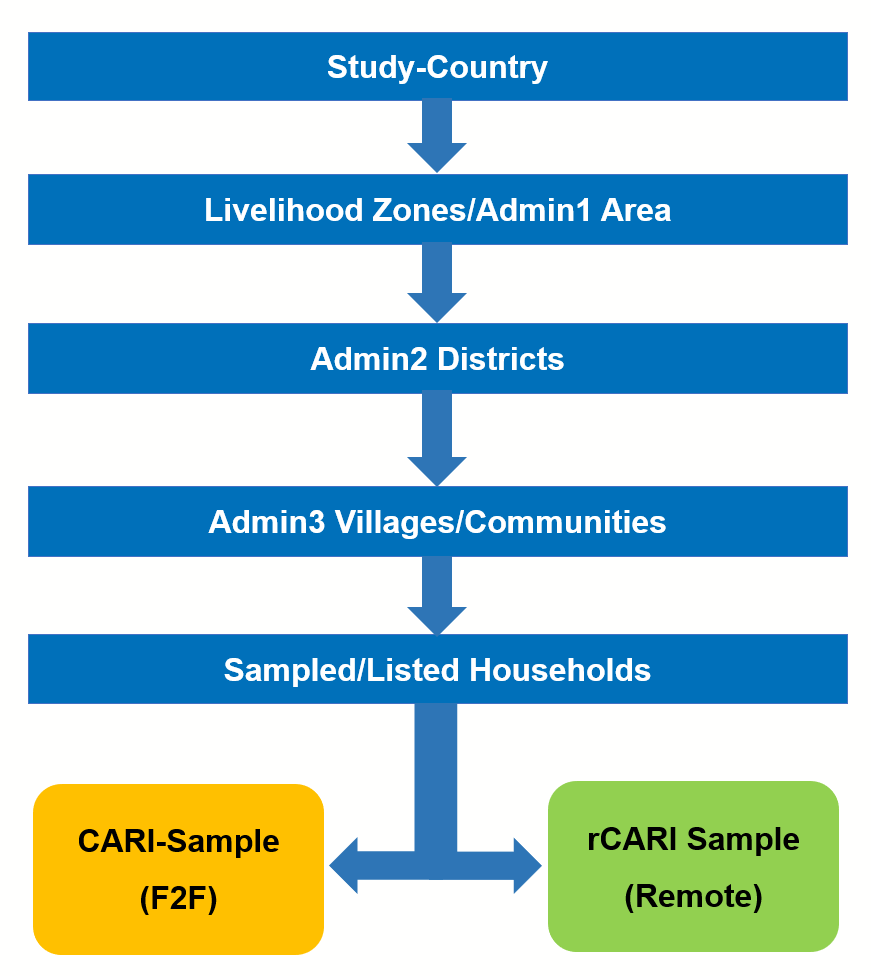
\includegraphics[scale=.75]{2_figure/Sample_Frame.png}
		\end{center}
		\label{fig:Sample_Frame}
		\caption{Sampling and Randomization Procedure}
	\end{figure}
	
	The main steps followed in identifying and selecting the admin areas at the various stages are listed and explained below.
	
	\subsection*{Step 1 - Selection of ADMIN1 (Livelihood Zones)}
	The first stage involves the identification and selection of Admin1 or livelihood areas that meets the inclusion criteria. A minimum of 2 Admin1 areas will be purposively identified and selected (on the recommendation WFP country offices) based on phone coverage, food security situation and accessibility. If more than 2 Admin1 areas meet the inclusion criteria, a simple random approach will be used to select 2 areas.
	
	\subsection*{Step 2 - Selection of ADMIN2 }
	In the second stage, a minimum of 4 ADMIN2 areas are purposively selected (2 per ADMIN1 area based on the outcome of Step 1) from the ADMIN1 areas that have been identified and selected based on the same criteria used to select the ADMIN1 areas.
	
	\subsection*{Step 3 - Selection of ADMIN5 - (Lowest Admin areas i.e., villages)}
	After identifying and selecting the Admin2 areas, all villages (ADMIN5 areas) in the selected ADMIN2 areas that met the inclusion criteria set out in Step 1 are listed as primary sampling units (PSUs). A full census of PSUs will be conducted in each selected ADMIN2 area to ensure equal chance of selection once the inclusion criteria is met. A list of 40 PSUs will be randomly selected (distributed equally across the selected ADMIN1s from Step 1). The study sample (households) will be selected from these 40 PSUs (depending on the number villages that will be selected).
	
	\subsection*{Step 4 - Sampling of households (HHs)}
	The final stage of the sampling procedure involves conducting a full census of all households in the selected ADMIN 5 areas. The census list forms the sampling frame for the study in each village. Households for the study will be selected following a simple random sampling approach (in the absence of any recent household census, there will be a fresh census conducted by the CO team with support from HQ). The aim is to collect information from households that is as accurate and representative as possible in each study area. Thus, the idea is to give equal chance of selection to all households in each PSU as much as practicable. The study will therefore enlist an equal number of households, a minimum of 100 households per PSU taking into consideration previous attrition. Trained and conscientious enumerators will be used for the household selection process.
		
	To ensure the integrity and ethics of the study are maintained, informed consent will be taken from all households at the listing phase to ensure that all households understand and agree to participate in the study. Based on the number of PSUs per country, around 4000 HHs will be listed for the study. The full village census will be used as the sampling frame for the next stage	
	
	\subsection*{Step 5 - Randomization of household (HHs)}
	Consented final sampled households in Step 4 are randomly assigned into one of two survey modalities/groups; F2F (CARI group) and remote (rCARI group). The design is such that the sample will be divided equally between the two groups using a standardized randomization process. 
	
	Randomization will be be based on the baseline characteristics to ensure that households assigned to the two modalities are well balanced statistically to allow for comparability of the two groups.
	
	All interviews (both F2F \& remote) will be conducted simultaneously over the same time frame to ensure that households are reporting food security situation over the same window and also affected by similar geographical situations.
	
	% -------	
	\pagebreak
	% -------	
	
	\subsection{Mauritania pilot study}
	Mauritania is made up of 15 Administrative regions. Following the rCARI study framework in Figure 1, the CO has identified Guidimakha and Hodh Ech Chargi regions as the two ADMIN1s for the study implementation in Mauritania.
	
	These two regions have been selected primarily because of the phone coverage, diversity of livelihoods, food security distribution, and accessibility criteria. 
	
	\begin{figure}[H]
		\begin{center}
			
\includegraphics[scale=.75]{2_figure/MTN_Sampling.png}
		\end{center}
		\label{fig:MTN_Sample_Composition}
		\caption{Systematic sampling \& sample size in each ADMIN area}
	\end{figure}
	
	
	\subsubsection{ADMIN1 AREAS (2 Regions)}
	\begin{itemize}[left=2.0em]
		\item[1.] Hodh Ech Chargi region
		\item[2.] Guidimakha region
	\end{itemize}
	
	These Admin1 areas have been carefully selected (purposively) to based on the phone access, accessibility and food security situation. The food security is maps used are based on the latest Cadre Harmonise (CH) food security analysis conducted 2024. Furthermore, these are have been selected to capture households with varied and diverse livelihood activities as much as possible that would allow for the testing of the income choice and income change indicator. 
	
	
	\subsubsection{ADMIN2 AREAS (8 Districts)}
	In total eight ADMIN2s in total will be selected from the ADMIN1s i.e., 4 in Hodh Ech Chargi region and 4 from Guidimakha region. These selections was done with special consideration to allow for a mix of rural and urban households to also include livelihood activities prevalent in rural and urban Mauritania such as formal employment, self-employment and agricultural activities. The ADMIN2 selected are listed below.
	
\textbf{Guidimakha Region}
	\begin{itemize}[left=2.0em]
		\item[1.]Ould Yenge
		\item[2.]Selibabi 
		\item[3.]Wompou	and, 
		\item[4.]Ghabou
	\end{itemize}
\textbf{Hodh Ech Chargi Region}
	\begin{itemize}[left=2.0em]
		\item[1.]Bassikounou 
		\item[2.]Nema  
		\item[3.]Timbedra and, 
		\item[4.]Djigueni 
	\end{itemize}
	
	
	\subsubsection{ADMIN3 AREAS (8 Communes)}
	A total of eight ADMIN3 areas (communes) are then selected also spread out equally in each of the the ADMIN1s  selected i.e., 4 in Hodh Ech Chargi region and 4 from Guidimakha region. The same criteria as employed in identifying ADMIN2s is used to select the communes. For a full list of all the ADMIN level areas selected with the population as at the last census (2023), see Table 1.
	
	\subsubsection{Selection of ADMIN5 Areas (40)}
	
	The actual selection of Admin5 areas has been done after an audit of actual mobile phone coverage and penetration which done in collaboration with the telephone companies operating in Guidimakha and Hodh Ech Chargi regions.
	
	Due to the sparsely population distribution in Mauritania, more ADMIN5s (villages) will be sampled in order to achieve the sample size. The recommendation of the CO VAM team is to purposively select 40 village in total. 
	It must be mentioned that, the study does not consider dependency among households at the village level to be a significant issue, as the primary focus is on comparing survey modalities rather than generalizing findings. Furthermore, the study villages would be purposively selected to reflect diverse contexts, and also households within each village will be randomly sampled to ensure varied representation.

	\begin{table}[!ht]
	\caption{List of Selected ADMIN Areas and Population Estimates (2023 Census) - MTN Pilot}
	\centering
	\begin{adjustbox}{max width=\textwidth}
	\begin{tabular}{lllll}
		\hline 
		\scriptsize
		\textbf{Region} & \textbf{District} & \textbf{Commune} & \textbf{ADMIN5NAME(Village)} & \textbf{Population} \\ \hline\hline
		~ & Bassikounou & Vassala & Mbera 2 &  3,158  \\ 
		~ & (116,818) & (75,585) & Diouweinkara &  2,524  \\ 
		~ & ~ & ~ & Kendierla &  1,287  \\ 
		~ & ~ & ~ & Kousana &  1,271  \\ 
		HODH CHARGUI & ~ & ~ & Leghdhaf &  874  \\ 
		~ & ~ & ~ & Elkheir Elgani &  1,140  \\ 
		~ & Nema & Nema & Sedra &  262  \\ 
		~ & (116,418) & (35,000) & ~ & ~ \\ 
		~ & Timbedra & Timbedra & Dahara &  829  \\ 
		~ & (108,525) & (33,792) & Bira &  767  \\ 
		~ & ~ & ~ & Magham Ehel Etar &  419  \\ 
		~ & ~ & ~ & Leghweirga &  258  \\ 
		~ & ~ & ~ & Breidili &  244  \\ 
		~ & Djigueni & Djigueni & Zeweirat Hassi Etleih &  3,112  \\
		~ & (89,498) & (21,618) & Mint Hmeidett 1 &  1,126  \\ 
		~ & ~ & ~ & Agueil &  445  \\
		~ & ~ & ~ & Oum Arzika 3 &  360  \\ 
		~ & ~ & ~ & Akhwal Eliyil &  334  \\ \hline
		\textbf{EXPECTED SAMPLE FRAME} \\ \\ \textbf{HODH REGION} & ~ & ~ & ~ &  \textbf{18,410}  \\ \hline \hline
		~ & Ghabou & Gouraye & Gouraye &  3,262  \\ 
		~ & (112,563) & (34,761) & Boutenda &  2,209  \\ 
		~ & ~ & ~ & Zneigui Foulbé &  2,104  \\ 
		~ & ~ & ~ & Samba Kandji &  1,551  \\ 
		~ & ~ & ~ & Moudji 2 &  955  \\ 
		~ & Selibabi & Selibabi & Mbeighirett Bilal &  1,079  \\ 
		~ & (98,643) & (44,838) & Toumbou &  397  \\ 
		~ & ~ & ~ & Mbeighirett Sahaba &  357  \\ 
		GUIDIMAKHA & ~ & ~ & Mbeighirett Salam &  311  \\ 
		~ & ~ & ~ & Mborobé &  298  \\ 
		~ & Ould Yenge & Dafort & Verkaka &  541  \\
		~ & 91,275 & 21,015 & Ndaw Demba Mory &  560  \\ 
		~ & ~ & ~ & Bouguerba 2 &  1,050  \\ 
		~ & ~ & ~ & Garva Ehel Eljeilani &  977  \\ 
		~ & ~ & ~ & Lefkarine &  880  \\ 
		~ & ~ & ~ & Dara Doussou &  775  \\ 
		~ & Wompou & Ajar & Ejar Soninké &  2,307  \\
		~ & (57,443) & (9,381) & Ejar Ehel Ali &  1,348  \\ 
		~ & ~ & ~ & Chelkha Elbeidha &  805  \\ 
		~ & ~ & ~ & Ejar Peul &  772  \\ 
		~ & ~ & ~ & Eljedida &  684  \\ 
		~ & ~ & ~ & Wendou Seno &  481  \\ 
		~ & ~ & ~ & Eljedida &  1,811  \\  \hline
		\textbf{EXPECTED SAMPLE FRAME} \\ \\ \textbf{GUIDIMAKHA REGION} & ~ & ~ & ~ &  \textbf{25,514} \\ \hline \hline
		\end{tabular}
	\end{adjustbox}
	\begin{tablenotes}
		\item Note: Population of ADMIN2 and ADMIN3 are stated in brackets
	\end{tablenotes}
\end{table}
	\label{tab:ADMIN5_MTN}
	
	\subsubsection{Selection of respondents (Households)}	
	The sampling frame will include all households within the selected ADMIN5 areas (PSUs). The household sampling process will involve several steps. First, a complete census of all households in the chosen ADMIN5 areas will be conducted to compile a comprehensive household list for each area. During the census, baseline demographics and socioeconomic characteristics of each household will be recorded, and mobile ownership and network coverage within each household will be assessed to ensure that only households with mobile access are included in the final sampling frame. The sampling frame for each PSU will therefore consist of households that have consented to participate and possess mobile phones.
	
	Trained and conscientious enumerators will conduct the household census in each PSU using a standardized questionnaire. All households will be contacted to obtain participation consent, and baseline characteristics will be collected, along with phone numbers and GPS locations, to facilitate identification for follow-up face-to-face interviews.
	
	The final sampling frame will include only households that have consented, have access to mobile phone, and completed the listing questionnaire. The actual study participants will then be selected through a simple random sampling process based on the finalized census list of households that meet the inclusion criteria. Approximately 115 households will be randomly sampled from each village (averaging about 4500 households in total).
	 
	\subsubsection{Randomizing the study sample}
	Households that do not have access to mobile phones or phone coverage will be dropped before the final randomization. Similarly, households with incomplete baseline and contact information will be dropped from the sample before randomization. The final household randomization will be done independently by ADMIN5 separately. This is to ensure comparability in the livelihood answers that will be reported across modalities in each ADMIN5 area.
	
	\begin{figure}[H]
		\begin{center}
			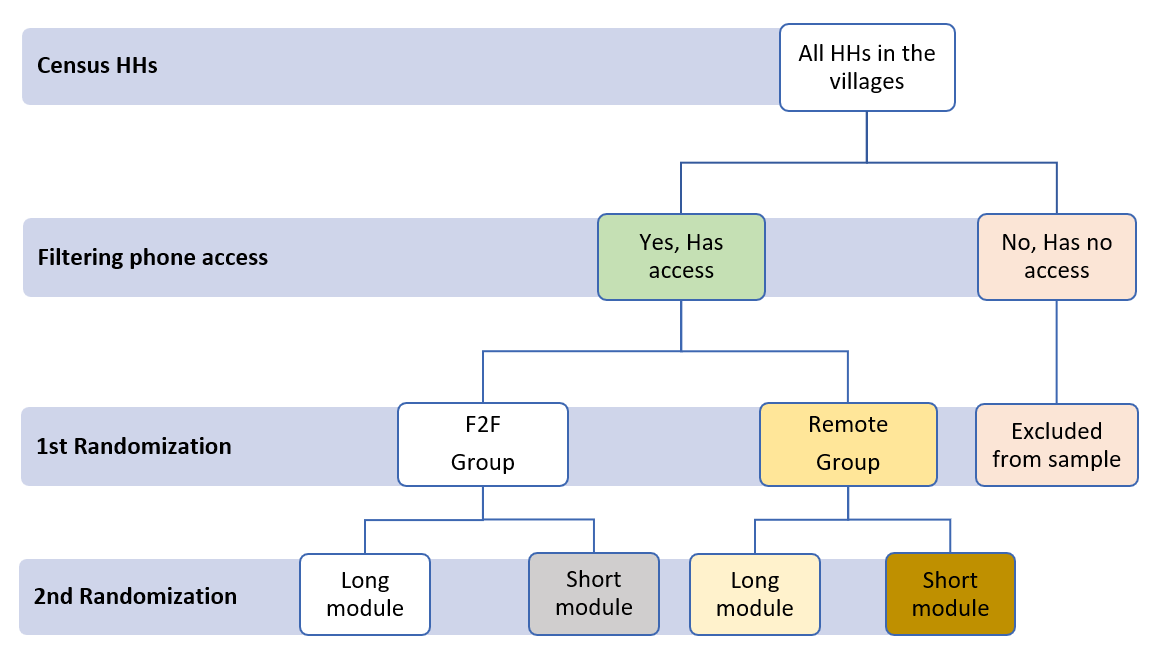
\includegraphics[scale=.70]{2_figure/MTN_Randomization.png}
		\end{center}
		\label{fig:Sample_Randomization}
		\caption{Step by step randomization of the survey sample}
	\end{figure}
	
	\pagebreak
	%----------
	\subsection{Training \& assignment of enumerators}
	
	To be qualified to be engaged as an enumerator for both the listing and data collection, all potential enumerators should have; 
	\begin{itemize}[left=2.0em]
		\item [1.] At least a university degree,
		\item [2.] First hand knowledge of the study areas (must speak the local language/dialect), and 
		\item [3.] Prior data collection experience (at least must have been involved in two separate food security surveys) in Mauritania. 
	\end{itemize}
	
	To ensure consistency in data collection, a 5-day in person training will be organized for both F2F and remote enumerators. The enumerator training will be conducted jointly by the Mauritania CO (VAM team), RBD and rCARI team from HQ. Training will be largely conducted in French, the predominant language of the study area. Local dialects will be used in cases where required to increase comprehension.
	A day's hands-on field pilot will be conducted at the end of the training session to test both the practical knowledge of enumerators and interview instruments for both cohorts (F2F and remote).
	A comprehensive field guide translated into French will be prepared at the end of the enumerator training. This will be provided to all enumerators to serve as quick reference in the field when they are in doubt. In addition, field supervisors with adequate understanding of food security and livelihoods of the study area will be engaged to work closely with all enumerators in the field to increase data quality.
	
	\subsection{Possible limitations of the design \& suggested mitigation strategies}
	
	Although a lot of thought has been given to the methodological design of the study, it must be mentioned that there remain some potential unavoidable sources of biases in the current experimental design setup. The potential sources and how the current design would remedy or reduce them are discussed below. 
	
	\textbf{1.} Lack of national representativeness of the survey. One of the key limitations of the methodology is its lack of nationwide coverage which is likely to affect the generalization of the results. However, given that the main objective of the study not to report national food insecurty but rather to test the two modalities within the same sample of respondents, the sample design has been adapted in such a way to ensure that the study sample will be as representative of the different food security groups and also that he households in the two cohorts are statistically comparable as much as possible. This will ensure the testing of the two modalities using the same sample and context.
	
	\textbf{2.} Possible lack of geographical variation in the distribution of actual respondents. With the phone survey likely to have lower response rate than F2F, there is a likelihood that completed surveys may be skewed in favour of F2F group which can affect the final analysis. To address this limitation and ensure that the final interviewed sample is large enough to allow for statistical analysis, a number of strategies will be adopted. First, the study will only be rolled out in areas that allow for both F2F and remote surveys. Second, a comprehensive household census (pre-survey phase) has been incorporated to ensures that we are able to achieve a uniform pre-survey distribution of both F2F and remote households. Third, increase sensitization of the study regions during the household census exercise. For example, during the census exercise, enumerators will pre-inform all households in selected villages about the study and its objective. Enumerators will also be tasked to ask all households for the appropriate time(s) of the day they could be contacted for the survey (both F2F and remote but this is particularly important for the remote interviews). Forth, increase the number of follow-up in the remote cohort. Specifically, in addition to the stated time by respondents to contacted, 3 additional time windows, i.e., mornings, afternoons and evenings will be used to make calls. This will ensure that more households are reached within the survey period. 
	
	\textbf{3.}	Confounding through enumerator effects (gender, training and motivation). Given that both survey cohorts are to be collected simultaneously, the same enumerator cannot be used to collect both cohorts which can inadvertently influence the results. To address this potential bias, randomization will be adopted when assigning enumerators to the PSUs and modalities (a minimum of two enumerator will be assigned to each PSU). Also, to ensure equivalence of comprehension of the questionnaire across all enumerators, F2F and remote enumerators will be trained together by the same facilitators. Also, knowledge test will be conducted at the end of the enumerator training with the lowest scoring enumerators being or retrained or dropped all together. Finally, daily high frequency checks will be put in place by the data management team to access the performance of each enumerator. Those with enumerators recording questionable data consistently will either be asked to re-conduct the interviews or dismissed all together where the issues persist. Finally, conscious efforts will be made to increase the number of female enumerators conducting the remote interviews (evidence show that female enumerators tend to achieve higher response rates compared to males in phone survey).
	
	\textbf{4.} Possible high attrition particularly in the remote cohort affecting statistical analysis. To minimise this limitation, the sample size has been increased to 4500 households in Mauritania. This is expected to create adequate allowance to take care of sample attrition resulting form network issues, refusals and lack of access.
	\textbf{5} Issue of dependencies for selected households. Based on the broad objective and design of the study, dependency may be considered less significant in this study for the following reasons.
	\begin{itemize}
		\item The study does not aim to generalize findings to a larger population but rather a pilot to that focuses on comparing survey modalities (e.g., F2F vs. remote).
		\item The design or analysis ensures sufficient diversity across clusters (i.e., villages), with the aim to minimizing the impact of dependency if any.
	\end{itemize}
	
	While the assumptions about dependency are appropriate for this pilot study, analysis aiming for population-level generalizations may need to account for clustering effects more rigorously.
	
	
	
\end{document}